\chapter{State of the art}

In this chapter we introduce the theory of level design; we examine how the problem is being tackled for singleplayer and multiplayer first person shooters both by the industry and the academical research. \\
We then proceed to analyze \textit{Procedural Content Generation} (PCG) and, specifically, \textit{Search-Based Procedural Content Generation} (SB-PCG) to generate and evaluate new content and, specifically, new maps for videogames, focusing on the research for FPS. \\
Lastly, we consider the concept of video game difficulty, with a particular focus on how multiplayer games and how maps can affect it. \\

\section{Level design theory}

\textit{Level design} is the discipline concerned with the creation of video game levels. Starting from a game concept, the level designer is tasked to build environments that explore the game concept by proposing challenges to the player. In this sense, the level designer is the one that transforms the simple game idea into something tangible.

\textit{Level design} is a fundamental task in the development of a game and it’s now extremely common to have figures specialized in this function. However, level design is not a well defined process yet: due to the level of imagination, trial and error and user input requested, it’s not easy to understand what the fundamental steps to achieve a good level design are \cite{the_invisible_hand}. 

In the years there have been researches aimed at finding common strategies to tackle level design, but often those researches are quite limited in scope since they consider a single genre of game (and often not covering it completely) and tend to get obsolete quickly due to the fast evolution of game and the introduction of new dynamics. Consider for example a game like Fortnite\footnote{People Can Fly, 2017}, a third person shooter which uniquely allows players to build structures that can be used as covers or look-out point. The introduction of a single dynamic (altering the map topology) completely changes the way level design has to be tackled, potentially invalidating other techniques used for other, more traditional third person shooters.

Despite this, there are some core ideas and techniques behind level design which remain valid no matter what, such as the level flow. In single player and cooperative multiplayer games, the level flow is defined as the series of action and movements that the player needs to perform to complete a level. The quality of a level flow can be measured in different ways, for example by checking whether the players ever felt lost or overwhelmed or by measuring how often the various game dynamics are used in a satisfying way.
There are various ways to guide the user according to the level flow: sound, architecture, items, collectibles, lightning, illumination, color coded conventions are all examples of resources that a level designer can use to guide the user along the correct path. 

\begin{figure}[hbpt]
\centering
  
\includegraphics[width=0.8\linewidth]{Images/images/stanley_parable.png}
  \caption[Usage of lighting is The Stanley Parable]{In this section of \textit{The Stanley parable}\footnotemark, a game known for playing with and deconstructing common gaming tropes, lighting is used to great effect to guide them through the \textit{Mind Control Facility} room, distracting them from the "Escape" path marked on the left.}
  \label{fig:stanley_parable}
\end{figure}
\footnotetext{Galactic Cafe, 2013}

A brilliant example of this is Mirror’s Edge \footnote{Digital Illusions CE, 2008.
}, which uses a really clear color code, with red highlighting interactable objects in an otherwise white world, to guide the player through its fast-paced levels. There are also even more inventive solutions, like the dynamic flock of birds in Half-Life 2\footnote{Valve, 2004.}, used to catch the player attention or to warn him of incoming dangers \cite{half_life_2}.

% Finally, sounds and architectures are other elements that can be used to guide the player. In the academic environment, a lot of researchers have analyzed the effectiveness of this kind of solutions: Alotto[4] considers how architecture influences the decisions of the player, whereas Hoeg[5] also considers the effect of sounds, objects and illumination, with the last being the focus of Brownmiller’s[6] work. %In competitive multiplayer games the level flow is defined by how the players interact with each other and with the environment. Given that the objective is no longer to complete a level but to beat the opponents, in this kind of games there is no specific path to guide the player to, so the influence that the level designer can exert is much more limited and most of the control comes from the map design and the placement of elements. Güttler et al [Christian Güttler e Troels Degn Johansson. ‘Spatial Principles of Level design in Multi-player First-person Shooters’]. studied spatial design and gameplay evolution of various multiplayer maps and identified what they call “collision points”, the spots where the majority of conflicts occur. By carefully placing spawn points and collectible and designing the connectivity of the map (e.g. choke points and open areas), a level designer can partially control where this collision points will occur, thus influencing the level flow.

In competitive multiplayer games the level flow is defined by how the players interact with each other and with the environment. Given that the objective is no longer to complete a level but to beat the opponents, in this kind of games there is no specific path to guide the player to, so the influence that the level designer can exert is much more limited and most of the control comes from the map design and the placement of elements. Güttler et al \cite{spatial_principles_level_design} studied spatial design and gameplay evolution of various multiplayer maps and identified what they call “collision points”, the spots where the majority of conflicts occur. By carefully placing spawn points and collectible and designing the connectivity of the map (e.g. choke points and open areas), a level designer can partially control where this collision points will occur, thus influencing the level flow. 

In the academic world, level flow for single and multiplayer games has been researched, although not as extensively as it could have. Nonetheless, some interesting results were obtained by some studies. 
For example, Larsen \cite{larsenleveldesignpatterns} analyzes three really different multiplayer games, Unreal Tournament 2004\footnote{Epic Games
Digital Extremes, 2004}, Day of Defeat: Source\footnote{Valve, 2005} and Battlefield 1942\footnote{Digital Illusions CE, 2002} and identified shared patterns, measuring their effect on gameplay in order to suggest some guidelines for their use. Some of the patterns, for example placing highly values resources and items in risky places  to balance their effectiveness with the danger of collecting them, are generic enough to be universal for all games of the genre and not. 

Hullet and Whitehead \citep{design_patterns_fps} instead managed to identify shared patterns between single and multi player FPS and additionally Hullet \cite{science_level_design} managed to prove cause-effect relationships for some of this patterns by confronting hypothesized results with the ones observed on a sample of real players.


\section{Procedural content generation}

\textbf{Procedural content generation} (PCG) is a method of creating content algorithmically as opposed to manually, typically through a combination of human-generated assets and algorithms coupled with computer-generated randomness and processing power.

In game development, PCG allows to easily create new assets, maps, levels and even, in some niche cases, music and dialogue.

One of the first notable usages of PCG is \textit{Rogue}\footnote{Michael Toy, Glenn Wichman, 1980.}, a exploration survival game where maps, monsters, items and the like are all randomly generated. Rogue has been so influential that a whole genre of game, called roguelikes, was born and even today games of this type, like Pokémon Mystery Dungeon: Rescue Team DX\footnote{Spike Chunsoft, 2020}, are still being developed following more or less the same basic principles.

PCG then continued to be used extensively as a way to overcome the otherwise limited memory available to systems at the time, sometimes with great effect: The \textit{Elder Scrolls II: Daggerfall}\footnote{	Bethesda Softworks, Flashpoint Productions, 1996} for example featured a map as big as Great Britain and the space exploration game \textit{Elite}\footnote{David Braben, Ian Bell, 1984} could in theory contain 282 trillion galaxies, but only 8 where present in the final product.
Due to the massive scale of content generated by PCB in this way, it was impossible to fully check the quality of the contents generated, which in some situations where simply unplayable. 

With time, thanks to the increase in computational and memory resources, PCB stopped being used to overcome system limitations but continued to be a very useful tool for different reasons.

First, PCG allows developers to cut production costs, both in AAA and low-budget games, by automatizing generation of some contents and assets. Consider for example SpeedTree\footnote{\url{https://store.speedtree.com/}}, a middleware tool capable of procedurally generating a plethora of plants, bushes and all kinds of vegetation or World Machine\footnote{\url{http://www.world-machine.com/}}, another middleware capable of producing realistic looking environment terrains.

\begin{figure}
\centering
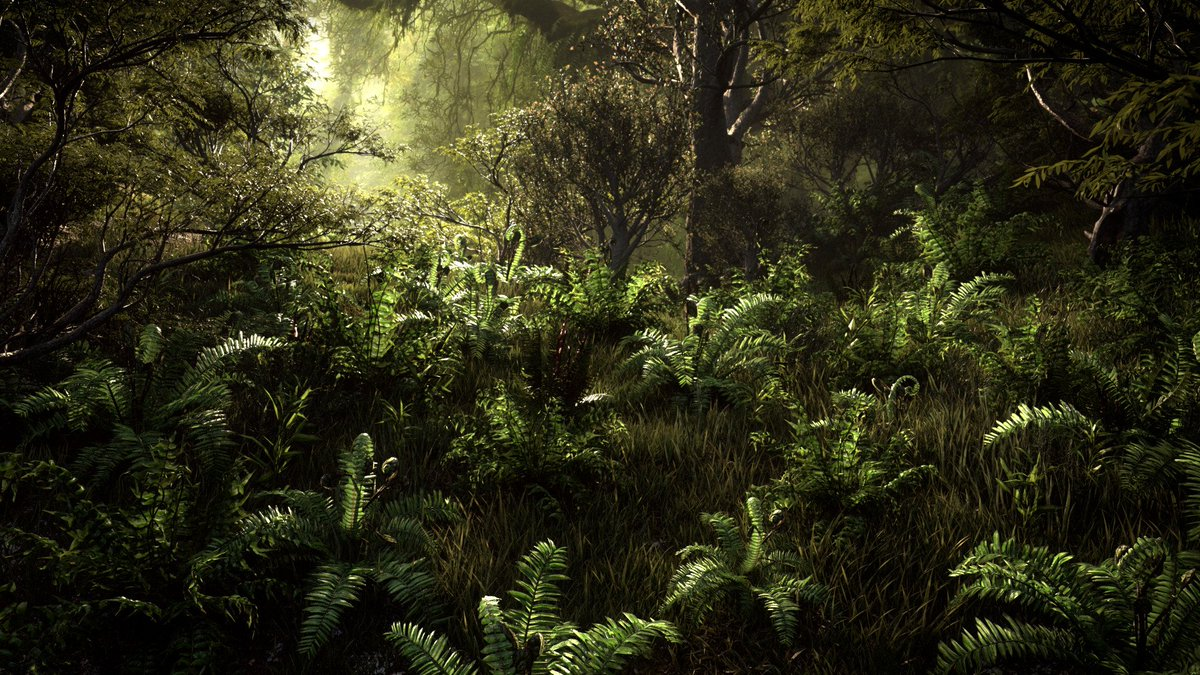
\includegraphics[width=0.8\linewidth]{Images/images/SpeedTree.jpg}
\caption{An example of environment filled with vegetation generated using \textit{SpeedTree}}
\end{figure}

Second, PCG can be used to increase replayability of games by creating new contents, missions, etc. For example, \textit{The Binding of Isaac: Rebirth}\footnote{Nicalis, 2013.} changes map layout and collectibles every match, therefore giving the ability to play a completely different match every time.

Lastly, PCG is so flexible that the whole concept of the game can revolve around it. The prime example of this is No Man’s Sky\footnote{Hello Games, 2016}, an exploration game where the whole world is generated with PCB, resulting in more than 18 quintillions\footnote{Specifically, 18.446.744.073.709.551.616 planets}  planets to explore, each with its own flora and fauna. Another great example is the Borderlands\footnote{Gearbox Software} series, where weapons are generated randomly by piecing together different parts, resulting, in the case of the first game, in more than 17,750,000 unique weapons.

\subsection{Procedural content generation with search algorithms}
PCG has attracted more and more academic interest in the years and many researches have been conducted to try and push PCG even further. While currently PCG techniques are rather simple and limited in scope, researches have been conducted to try to devise more elaborate generation algorithms and procedures to create more interesting content. This increased complexity however leads to a new challenge: evaluating the quality of the what is generated. 

The simplest approach, called \textbf{constructive PCG}, consists of, after generating content which passes some simple verification tests, letting a human decide whether the generated content is suitable for its purpose. 

%TODO Lanzi non aveva mostrato un sistema di generazione di tracce per un gioco di corsa dove all’utente venivano mostrate 8 mappe diverse e poteva scegliere la sua preferita, dettando così l’evoluzione? Potrebbe essere un esempio da mettere qui.

The problem of constructive PCG is that, by having a human in the equation, the entire process slows down and it’s impossible to exploit the full speed and generation capabilities of computers. For this reason the academic world is investigating a different approach for PCG, based around search algorithms and named \textbf{generation-and-test} or \textit{optimization-based PCG}, which attempts to automate the evaluation of the content to remove humans from the equation until possibly the very end of the process.

\textit{Generation-and-test} PCG is based around the fundamental concept of \textbf{fitness function}: a procedure used to evaluate how good a given content is for the purpose desired by assigning a real value or vector of real value representing its fitness. How the fitness function evaluates the quality of the content is an ad-hoc problem discussed in \Cref{section:fitness_function}. The fitness value assigned to each item is used to guide the generation process: individuals with higher scores have more influence over the generation of new ones. In this way, with time new contents will tend to have higher fitness values.

Using the fitness values to improve upon previously generated contents requires using a search algorithm, which allows us to scan a portion of the search space, representing the entirety of contents which can be created by the PCG procedure, in an attempt to find the highest valued content. 
The search algorithms used are often part of the larger family of \textbf{Evolutionary Algorithms} (EA): procedures which emulate natural biological evolution schemes, such as reproduction and mutation, to explore the research space.

When combining PCG and EA, the resulting procedure starts from an initial set of candidates, called \textit{population}, usually selected randomly and representing in some way the content to be evolved. 

Evolution happens in cycles, called epochs. Each epoch starts by a evaluating the \textit{fitness function} for each individual currently in the population. The fitness values computed are then used by the algorithm to choose which elements should be discarded and which ones should be preserved in the next epoch in a process called selection. After the selection, the surviving individuals can be kept as is, bred with others by employing cross-over or changed by using mutation in order to generate totally new individuals. The population obtained at the end represents the next generation and is the starting point for the process in the for the next epoch.

This process can be executed again and again, slowly exploring the search space until some stopping conditions, such as reaching the maximum number of epoch, finding a individual with a particularly high fitness value or loosing too much variance in the population, are met.

For a more detailed description of EA, interested readers can consult \cite{essentials_of_metaheuristics} and \cite{ea_critical_review}.

EA cannot usually work directly with the final content representation, be it a map, 3D model or anything else, it instead needs to use some encoded representation of the item. For this reason, in EA two concepts, again taken from biology, are introduced:
\begin{itemize}
\item \textbf{Genotype}: The low-level representation of the individual, the genotype encodes the individual as a set of parameters and values (e.g. string of bits, set of numbers) and is used by the evolution algorithm cross-over and mutation processes.
\item \textbf{Phenotype} The high-level representation of the individual, the phenotype is the actual content that is going to be generated and it’s the final product on which the fitness function is evaluated.
\end{itemize}

These two representation aren’t disjointed: there must be a way to map a genotype to the related phenotype in order for the evolution algorithm to work. Choosing a good genotype representation for the map and a valid mapping function from genotype to phenotype are two crucially important steps in preparing an EA,
since from those depends how efficiently the algorithm can explore the research space \cite{sbpcg_taxonomy}.

Using a genotype with too many parameters expands the search space, making it more likely to contain the optimal content to generate but causing the algorithm to converge to optimal solutions very slowly; on the contrary, too little parameters allow fast conversion but removes many potentially good elements from the search space. Finding a good balance is a complex problem named \textit{curse of dimensionality}\footnote{\url{https://en.wikipedia.org/wiki/Curse_of_dimensionality}}.

\subsection{Fitness function}
\label{section:fitness_function}
Using EA with PCG requires defining some key parts of the search algorithm, like the \textit{selection}, \textit{cross-over} and \textit{mutation} operators and the fitness function. Among those, the first three are usually relatively easy to define since many different techniques have already been studied and can be recycled for the problem at hand.

Defining a \textit{fitness function} instead is a complex, domain specific problem for which ad-hoc solutions must be devised. The main challenge to tackle is finding a clear correlation between parameters that can be measured by the function and what the user is trying to achieve by employing the EA; for example, measuring how strong or weak a specific generated weapon is is fairly easy; measuring how much enjoyment a human player might get from playing a generated map is hard, if not impossible. 

In fact, finding the right way to map what a human might think of a specific content is the main challenge of SB-PCG but it’s necessary to find a way to do so since, as stated before, bypassing the problem by letting the humans themselves judge the content (constructive approach) slows down the evolution process, making it impossible to explore the search space quickly and efficiently.

Fitness functions can be classified based on how they compute the evaluation metrics \cite{sbpcg_taxonomy}, and in particular we can identify:

\begin{itemize}
\item \textbf{Direct fitness functions}: The generated content is scored directly based on parameters of the phenotype. As an example, computing the average visibility of tiles in a map is a direct fitness function.
\item \textbf{Simulation-based fitness function}: The generated content is scored by extracting metrics out of simulations run using it. As an example, simulating matches on a generated map can be a great way to determine some of its characteristics, such as balance, which play styles it favours (e.g. close-range combat vs long-range combat), etc. They are extremely useful when it’s not clear how to evaluate the quality of the content by looking at its characteristics alone, but at the same time introducing this simulation step slows down significantly the evolution and introduces the problem of finding ways to realistically replicate interactions with the generated content. 
\item \textbf{Interactive fitness function}: The generated content is scored by gathering feedback from human testers. This approach allows to get realistic feedback on the content generated but is usually discouraged given that involving human actors slows down the process. Usually, it’s best to use this as a final step to validate the results obtained by the evolution.
\end{itemize}

\subsection{Procedural content generation for First-person shooters}
PCG of maps for FPS has been the focus of many studies in the years. One of the first works in this sense comes from Cardamone et al \cite{cardamone_evolving_maps} which tried to understand which kinds of map generated more interesting gameplay. To do so, the authors generated, using EA, maps for Cube 2: Sauerbraten\footnote{Wouter van Oortmerssen, Lee Salzman, Mike Dysart, 2004} based on four different structural representations and, by simulating matches on them, extracting the average time per fight, defined as the duration of the time range starting from the moment a player starts combat with another until the moment one of the two dies or escapes. The idea behind this choice is that, the longer this period, the more possibilities the map offers to escape, take cover, recover health and, in general, enact tactical strategies that make the game more interesting.

This research lead to two interesting results: first, its actually possible to use EA to evolve playable maps and second, the map representation had noticeable effect on the final results, so that some genotypes were better suited for the objective.

Starting from these results, Stucchi \cite{stucchi_evoluzione} tried to use EA to generate balanced maps for one-vs-one matches starting from any combination of players skills and equipment, using entropy as a kill ratio entropy as a the fitness function. The results showed how maps evolved to adapt their structure to bring advantage to the disadvantaged/less skilled player.

Arnaboldi \cite{arnaboldi_framework}, starting from Stucchi's result and setup, increased the quality of the simulations by improving the AI of Cube 2 bots used to run the games. This demonstrated one intrinsic problem of simulation based fitness functions: the quality of the result depends on the quality of the actors running the simulations; in order to get realistic results, the bots should behave as close as possible to a human agent.

Another problem in Cardamone et al’s approach was raised by Ølsted et al \cite{olsted_interactive_evolution_competitive} who noted how their system generates maps unsuitable for team-based multiplayer FPS like Counter-Strike, where the game focus develops around specific objective placed across the map. The same authors also note how the maps do not respect so called “rules of good combat”, such as guaranteeing multiple alternative paths, and therefore propose a new map generation and evolution approach consisting of randomly selecting nodes on a grid and evolving corridors, rooms, pickups and respawns connecting them to optimize such rules. 
This approach, based on the analysis of some \textit{Counter Strike} and \textit{Call of Duty} maps, further differentiates from Cardamone, Stucchi and Arnaboldi researches by using an interactive fitness function, since bot behavior was not deemed sufficiently human-like. Some criticism on their method can be raised however, considering that users involved in the map evaluation provided a simple binary answer concerning their appreciation of the map, without analyzing in more detail gameplay results or map characteristics 

Yet another approach to solve the map generation problem was tested by Bhojan Anand and Wong Hong Wei in \cite{bhojan_hong_arena}, which leveraged PCG with search based algorithms to quickly generate maps for Capture and Hold\footnote{Game mode first appeared in Killzone 2 and 3 (Guerrilla Games, 2009, 2011) in which two teams compete for the control of some strategic points. Team score increases periodically based on the number of controlled points; the team with the most points at the end wins} in an online fashion. By interconnecting pre-existing tiles representing open, zones and inaccessible zones, maps are scanned to detect regions which are then connected and filled with respawn points, flags and cover points. As fitness function, the authors opted for a direct approach, by computing metrics based on connectivity of region, collision points, flag position balance, in this way the evolution can be extremely fast and maps could be computed in a matter of seconds. However, the quality of the results, due to lack of simulation, can be contested and for this reason the obtained maps where later tested by human players which provided positive feedbacks.

\section{Balancing difficulty in video games}
In designing and developing a video game, extra care should be taken to ensure that the game experience is coherent with the concept desired. In particular, given a set of elements and mechanics a game is based on, a game is balanced if there exist no dynamic that, due to flexibility, strength or any other factor, outshines all the others. 

In an imbalanced game, some of the game features are ignored in favor of the stronger ones, leading to an impoverishment of gameplay and a waste of design and development resources, since weaker mechanics are ignored.

When discussing balance of game elements and mechanics, two terms are often used: \textbf{overpowered}, when something is much stronger than the rest, even after accounting for any possible cost for its usage, and, on the contrary, \textbf{underpowered}, when something is too weak even at the lowest cost of usage \cite{game_balance_concepts}.

Balancing game has two very different objective depending on whether the game is single or multiplayer.
 
In single player, balancing consists of ensuring that the level of difficulty of the game is adequate given the intended target. For example, the Dark Souls\footnote{From Software} series is known for its unforgiving nature and therefore it is expected that their difficulty is much higher than the standard for games of that genre.

In multi player, balancing consists of ensuring that no player has any intrinsic advantage over the others and no game strategy dominates the other in all or almost all situations. For example, in the fighting game Super Smash Bros. Brawl\footnote{Sora Ltd., 2008}, \textit{Meta Knight}, one of the playable fighters, had to be banned from competitive play because he was excessively overpowered and the whole metagame\footnote{The metagame refers to the collective decisions that are made outside of a game that affect tournament play. A metagame is said to have a "shape" or "state" which refers to the commonly employed practices and strategies in tournaments} was forcibly evolving around finding ways to counter it.

\subsection{Balancing of multi-player games}
Given the focus on this thesis, we will now focus on balancing multiplayer games.

As stated above, the presence of \textit{overpowered} or \textit{underpowered} elements in a game tends to cause a shift in gameplay mechanics since players who discover this imbalance will start taking advantage to it, forgoing usage of the weaker alternatives. With time, more and more player will then start using this unbalanced element and switch to dominant strategies revolving around this element, making the game more and more one-dimensional and, ultimately, boring, given the lack of variety.

While ideally a game should not have any overpowered element (and this can be mostly achieved only during design phase), it’s also a valid alternative to have more than one overpowered element, in order to let players choose the mechanic to “abuse” while still ensuring a basic level of variety.
%TODO Add more?

\subsection{Balancing of maps in video games}
In first person shooter and real-time strategy games, one of the most important elements to balance are the maps on which the game takes place. Designing balanced maps is a complex process for which no standard exist yet. The general approach followed starts from a designer pitching a possible draft for the map. The map proposed is then tested by human players in order to gather feedback from them and extract gameplay data (such visited positions, death positions, etc.), both of which are used to improve the initial design and try again with a new pitch, in a manner similar to EA cyclical evolution.

The main problem of this process is devising the first ever idea for the map: a badly designed map will require many iterations to get a final, working result. Due to this, many studies have been conducted to understand at least what properties make it a good multiplayer map \cite{pascal_multiplayer}, \cite{epic_multiplayer}, \cite{dodger_multiplayer}, \cite{larsenleveldesignpatterns} in order to leverage them during the design phase. 

Burgun \cite{keith_multiplayer} in particular focused on balancing, arriving at the conclusion that even perfectly symmetric maps might not ensure balance because their structure might nonetheless advantage some some weapons or strategies. 

Despite all the research on map properties and a plethora of studies on balancing maps for RTS games, very few have studies balancing for FPS.

\section{Summary}
In this chapter we analysed the current state of level design for videogames, identifying the reason behind our and other similar researches on the topic.
We then looked at \textit{Procedural Content Generation} techniques used in the years to support game development or entirely replace some tedious works. We focused on PCG using search algorithms, describing how they work and how they can be applied to support generation of maps for First-Person shooters.
Finally, we looked at the concept of difficulty in video games and what it means to balance difficulty in different contexts.

